\begin{frame}{Motivation}{}
  \textbf{Question: How to use one algorithm to generate
    various (repeating) lattice pattern formations?}
  \begin{figure}
    \centering
    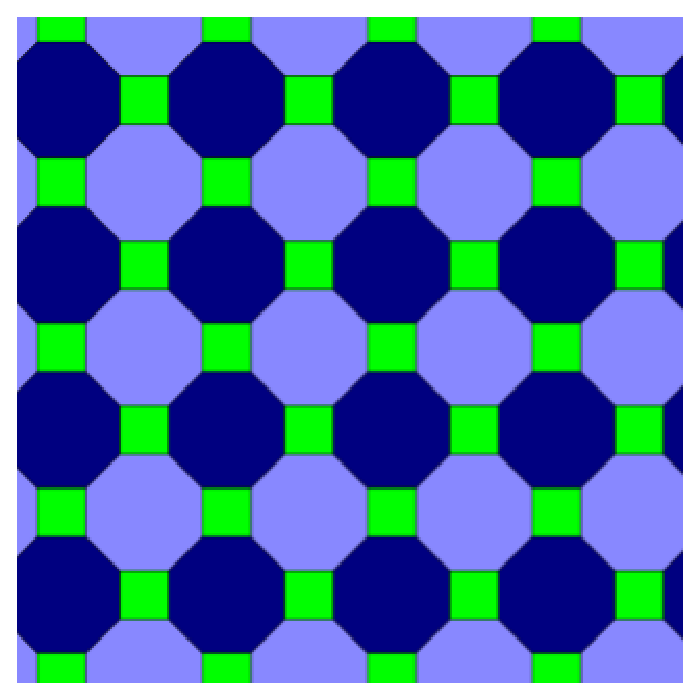
\includegraphics[height=1.8in]{figs/tessellation2}
  \end{figure}
  %% \begin{columns}
  %%   \begin{column}{.45\textwidth}
  %%     \begin{figure}
  %%       \centering
  %%       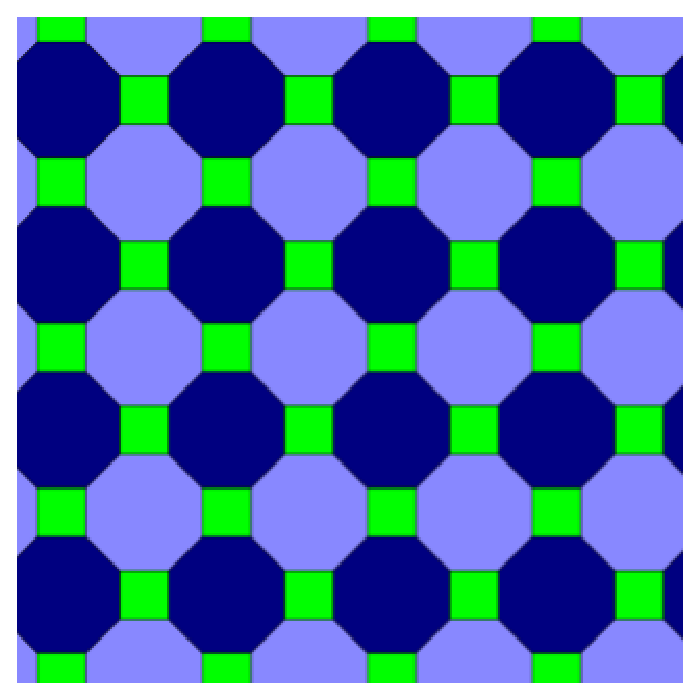
\includegraphics[height=1.5in]{figs/tessellation2}
  %%     \end{figure}
  %%   \end{column}
  %%   \begin{column}{.45\textwidth}
  %%     \begin{figure}
  %%        \centering
  %%        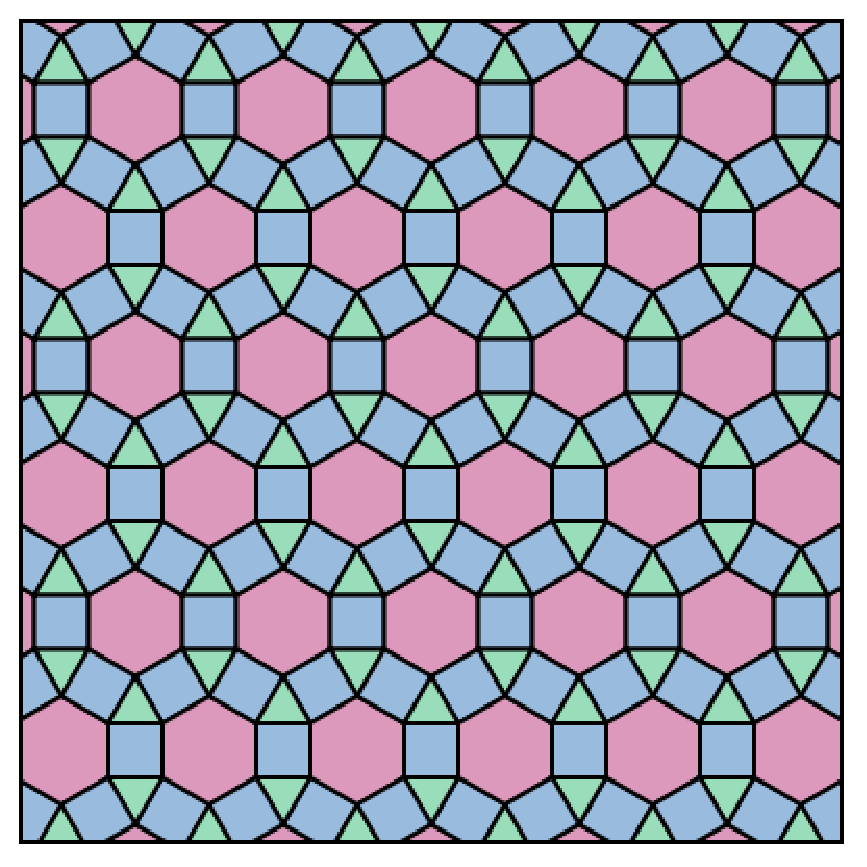
\includegraphics[height=1.5in]{figs/tessellation1}
  %%      \end{figure}
  %%   \end{column}
  %% \end{columns} 
\end{frame}
